
\subsection{Cloud Service}\label{subsec:cloud-service}

\subsubsection{Architektur}

Es gibt deren Domänen 2. Configuration und Notification.

So quasi als ob man 2 Microservices haben kann. Aber wär halt doof das für den stand jetzt schon so zu trennen, deshalb vorerst mal erst ein einzelnes.

\clearpage

\subsubsection{Domänenmodell}


Für die beiden Domänen gibt es natürlich auch so n paar Diagramme. Die gibts jetzt hier:


\subsubsection*{Domäne Configuration}

\begin{figure}[h]
    \centering
    \begin{minipage}[b]{1.0\textwidth}
        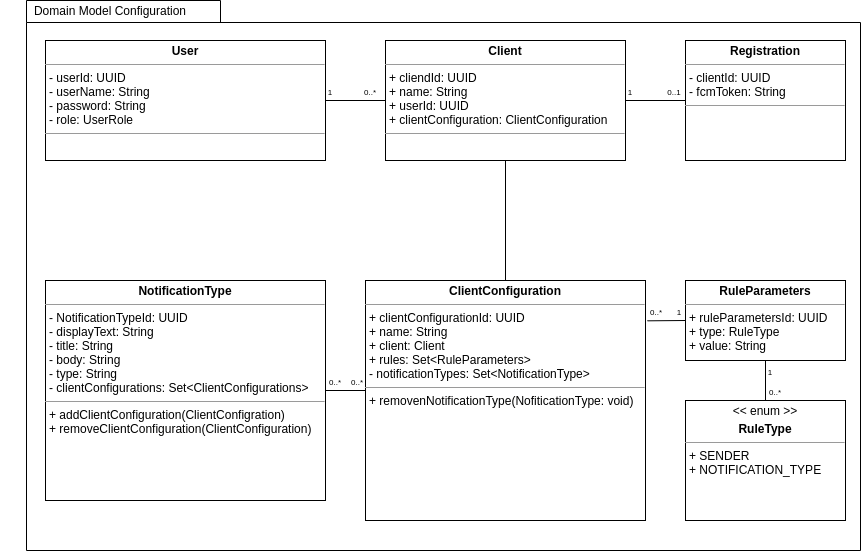
\includegraphics[width=\textwidth]{graphics/Class_Configuration_Domain}
        \caption{Domänenmodell Configuration}
    \end{minipage}
\end{figure}
Also erstmal gibts da son halb generischen konfigurationsmodel.
Wär auch fast mandantenfähig.
Aber halt nur fast.



\clearpage

\begin{figure}[h]
    \centering
    \begin{minipage}[b]{1.0\textwidth}
        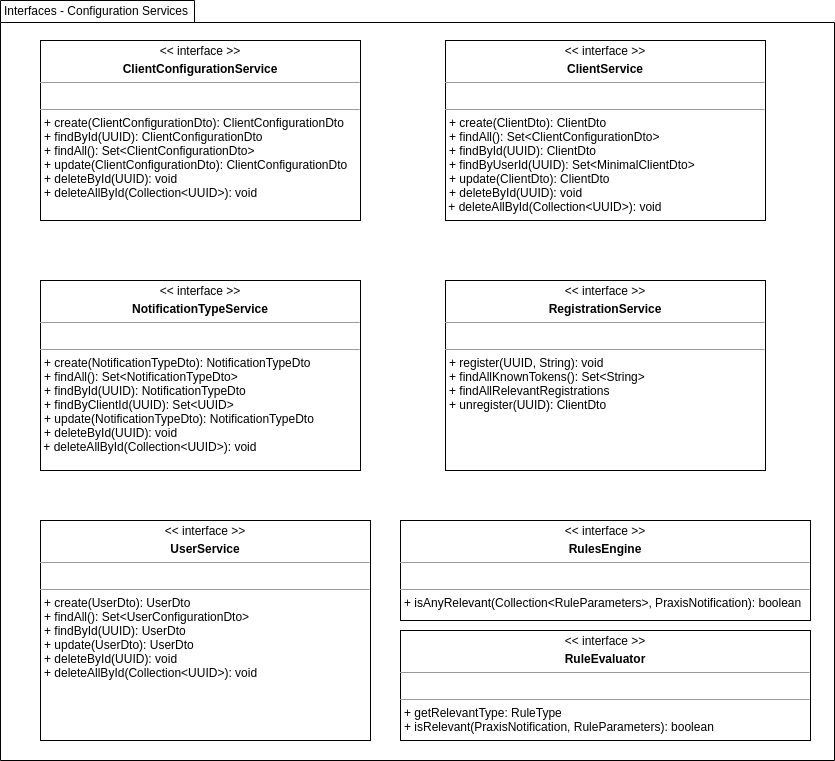
\includegraphics[width=\textwidth]{graphics/Class_Configuration_Services}
        \caption{Klassendiagramm Configuration Service Interfaces}
    \end{minipage}
\end{figure}
Services mit CRUD gibts hier.
Pro Service genau eine Instanz mit Default Prefix.
RulesEngine integration ist hier.
Details see Rules Engine.
Die RulesEngine sowie die RuleEvalautor Services werden ausschliesslich innerhalb der Applikation verwendet und sind nicht über die API zugreifbar.
Alle anderen Services bieten ihre Methoden über eine REST API an. Es wird darauf verzichtet, dass alles nochmal hier zu kopieren.
URL Konzept im Kapitel API.


\clearpage
Dann muss man ja noch sachen darauf auswerten können und zeug.
Das Bild zeigt: Strategy Pattern mit Spring is noch nice.

\begin{figure}[h]
    \centering
    \begin{minipage}[b]{1.0\textwidth}
        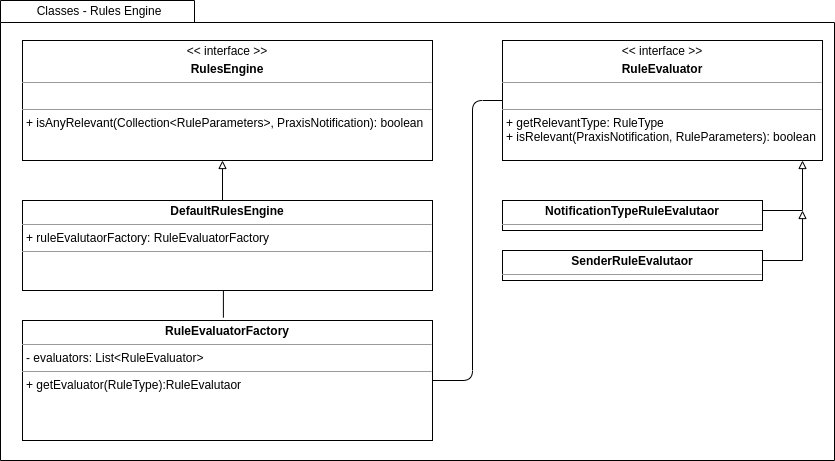
\includegraphics[width=\textwidth]{graphics/Class_Configuration_RulesEngine}
        \caption{Klassendiagramm Rules Engine}
    \end{minipage}
\end{figure}

\clearpage
\subsubsection*{Domäne Notification}

Joa, und die Notifikationen selbst muss ja auch noch wer verschicken.

\begin{figure}[h]
    \centering
    \begin{minipage}[b]{1.0\textwidth}
        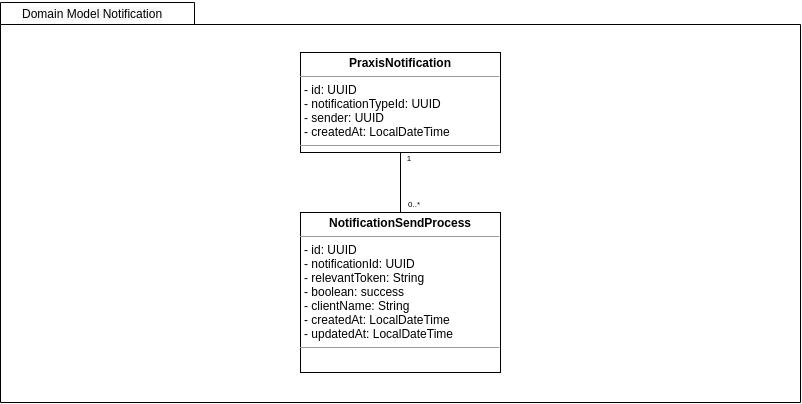
\includegraphics[width=\textwidth]{graphics/Class_Notification_Domain}
        \caption{Domänenmodell Notification}
    \end{minipage}
\end{figure}

Damit man weiss was passiert und teil Zeuch wiederholt werden kann.
Braucht dann klar auch noch n paar Services.




\clearpage
\subsubsection{API}

S gibt da n paar controller und die brauchen ein paar services.

\clearpage
\subsubsection{Laufzeitmodell}

\clearpage
